% Created 2022-12-16 Fri 15:57
% Intended LaTeX compiler: pdflatex
\documentclass[11pt]{article}
\usepackage[utf8]{inputenc}
\usepackage[T1]{fontenc}
\usepackage{graphicx}
\usepackage{longtable}
\usepackage{wrapfig}
\usepackage{rotating}
\usepackage[normalem]{ulem}
\usepackage{amsmath}
\usepackage{amssymb}
\usepackage{capt-of}
\usepackage{hyperref}
\graphicspath{{../../books/}}
% wrong resolution of image
% https://tex.stackexchange.com/questions/21627/image-from-includegraphics-showing-in-wrong-image-size?rq=1

%%%%%%%%%%%%%%%%%%%%%%%%%%%%%%%%%%%%%%
%% TIPS                                 %%
%%%%%%%%%%%%%%%%%%%%%%%%%%%%%%%%%%%%%%
% \substack{a\\b} for multiple lines text
% \usepackage{expl3}
% \expandafter\def\csname ver@l3regex.sty\endcsname{}
% \usepackage{pkgloader}
\usepackage[utf8]{inputenc}

% nfss error
% \usepackage[B1,T1]{fontenc}
\usepackage{fontspec}

% \usepackage[Emoticons]{ucharclasses}
\newfontfamily\DejaSans{DejaVu Sans}
% \setDefaultTransitions{\DejaSans}{}

% pdfplots will load xolor automatically without option
\usepackage[dvipsnames]{xcolor}

%                                                             ┳┳┓   ┓
%                                                             ┃┃┃┏┓╋┣┓
%                                                             ┛ ┗┗┻┗┛┗
% \usepackage{amsmath} mathtools loads the amsmath
\usepackage{amsmath}
\usepackage{mathtools}

\usepackage{amsthm}
\usepackage{amsbsy}

%\usepackage{commath}

\usepackage{amssymb}

\usepackage{mathrsfs}
%\usepackage{mathabx}
\usepackage{stmaryrd}
\usepackage{empheq}

\usepackage{scalerel}
\usepackage{stackengine}
\usepackage{stackrel}



\usepackage{nicematrix}
\usepackage{tensor}
\usepackage{blkarray}
\usepackage{siunitx}
\usepackage[f]{esvect}

% centering \not on a letter
\usepackage{slashed}
\usepackage[makeroom]{cancel}

%\usepackage{merriweather}
\usepackage{unicode-math}
\setmainfont{TeX Gyre Pagella}
% \setmathfont{STIX}
%\setmathfont{texgyrepagella-math.otf}
%\setmathfont{Libertinus Math}
\setmathfont{Latin Modern Math}

 % \setmathfont[range={\smwhtdiamond,\enclosediamond,\varlrtriangle}]{Latin Modern Math}
\setmathfont[range={\rightrightarrows,\twoheadrightarrow,\leftrightsquigarrow,\triangledown,\vartriangle,\precneq,\succneq,\prec,\succ,\preceq,\succeq,\tieconcat}]{XITS Math}
 \setmathfont[range={\int,\setminus}]{Libertinus Math}
 % \setmathfont[range={\mathalpha}]{TeX Gyre Pagella Math}
%\setmathfont[range={\mitA,\mitB,\mitC,\mitD,\mitE,\mitF,\mitG,\mitH,\mitI,\mitJ,\mitK,\mitL,\mitM,\mitN,\mitO,\mitP,\mitQ,\mitR,\mitS,\mitT,\mitU,\mitV,\mitW,\mitX,\mitY,\mitZ,\mita,\mitb,\mitc,\mitd,\mite,\mitf,\mitg,\miti,\mitj,\mitk,\mitl,\mitm,\mitn,\mito,\mitp,\mitq,\mitr,\mits,\mitt,\mitu,\mitv,\mitw,\mitx,\mity,\mitz}]{TeX Gyre Pagella Math}
% unicode is not good at this!
%\let\nmodels\nvDash

 \usepackage{wasysym}

 % for wide hat
 \DeclareSymbolFont{yhlargesymbols}{OMX}{yhex}{m}{n} \DeclareMathAccent{\what}{\mathord}{yhlargesymbols}{"62}

%                                                               ┏┳┓•┓
%                                                                ┃ ┓┃┏┓
%                                                                ┻ ┗┛┗┗

\usepackage{pgfplots}
\pgfplotsset{compat=1.18}
\usepackage{tikz}
\usepackage{tikz-cd}
\tikzcdset{scale cd/.style={every label/.append style={scale=#1},
    cells={nodes={scale=#1}}}}
% TODO: discard qtree and use forest
% \usepackage{tikz-qtree}
\usepackage{forest}

\usetikzlibrary{arrows,positioning,calc,fadings,decorations,matrix,decorations,shapes.misc}
%setting from geogebra
\definecolor{ccqqqq}{rgb}{0.8,0,0}

%                                                          ┳┳┓•    ┓┓
%                                                          ┃┃┃┓┏┏┏┓┃┃┏┓┏┓┏┓┏┓┓┏┏
%                                                          ┛ ┗┗┛┗┗ ┗┗┗┻┛┗┗ ┗┛┗┻┛
%\usepackage{twemojis}
\usepackage[most]{tcolorbox}
\usepackage{threeparttable}
\usepackage{tabularx}

\usepackage{enumitem}
\usepackage[indLines=false]{algpseudocodex}
\usepackage[]{algorithm2e}
% \SetKwComment{Comment}{/* }{ */}
% \algrenewcommand\algorithmicrequire{\textbf{Input:}}
% \algrenewcommand\algorithmicensure{\textbf{Output:}}
% wrong with preview
\usepackage{subcaption}
\usepackage{caption}
% {\aunclfamily\Huge}
\usepackage{auncial}

\usepackage{float}

\usepackage{fancyhdr}

\usepackage{ifthen}
\usepackage{xargs}

\definecolor{mintedbg}{rgb}{0.99,0.99,0.99}
\usepackage[cachedir=\detokenize{~/miscellaneous/trash}]{minted}
\setminted{breaklines,
  mathescape,
  bgcolor=mintedbg,
  fontsize=\footnotesize,
  frame=single,
  linenos}
\usemintedstyle{xcode}
\usepackage{tcolorbox}
\usepackage{etoolbox}



\usepackage{imakeidx}
\usepackage{hyperref}
\usepackage{soul}
\usepackage{framed}

% don't use this for preview
%\usepackage[margin=1.5in]{geometry}
% \usepackage{geometry}
% \geometry{legalpaper, landscape, margin=1in}
\usepackage[font=itshape]{quoting}

%\LoadPackagesNow
%\usepackage[xetex]{preview}
%%%%%%%%%%%%%%%%%%%%%%%%%%%%%%%%%%%%%%%
%% USEPACKAGES end                       %%
%%%%%%%%%%%%%%%%%%%%%%%%%%%%%%%%%%%%%%%

%%%%%%%%%%%%%%%%%%%%%%%%%%%%%%%%%%%%%%%
%% Algorithm environment
%%%%%%%%%%%%%%%%%%%%%%%%%%%%%%%%%%%%%%%
\SetKwIF{Recv}{}{}{upon receiving}{do}{}{}{}
\SetKwBlock{Init}{initially do}{}
\SetKwProg{Function}{Function}{:}{}

% https://github.com/chrmatt/algpseudocodex/issues/3
\algnewcommand\algorithmicswitch{\textbf{switch}}%
\algnewcommand\algorithmiccase{\textbf{case}}
\algnewcommand\algorithmicof{\textbf{of}}
\algnewcommand\algorithmicotherwise{\texttt{otherwise} $\Rightarrow$}

\makeatletter
\algdef{SE}[SWITCH]{Switch}{EndSwitch}[1]{\algpx@startIndent\algpx@startCodeCommand\algorithmicswitch\ #1\ \algorithmicdo}{\algpx@endIndent\algpx@startCodeCommand\algorithmicend\ \algorithmicswitch}%
\algdef{SE}[CASE]{Case}{EndCase}[1]{\algpx@startIndent\algpx@startCodeCommand\algorithmiccase\ #1}{\algpx@endIndent\algpx@startCodeCommand\algorithmicend\ \algorithmiccase}%
\algdef{SE}[CASEOF]{CaseOf}{EndCaseOf}[1]{\algpx@startIndent\algpx@startCodeCommand\algorithmiccase\ #1 \algorithmicof}{\algpx@endIndent\algpx@startCodeCommand\algorithmicend\ \algorithmiccase}
\algdef{SE}[OTHERWISE]{Otherwise}{EndOtherwise}[0]{\algpx@startIndent\algpx@startCodeCommand\algorithmicotherwise}{\algpx@endIndent\algpx@startCodeCommand\algorithmicend\ \algorithmicotherwise}
\ifbool{algpx@noEnd}{%
  \algtext*{EndSwitch}%
  \algtext*{EndCase}%
  \algtext*{EndCaseOf}
  \algtext*{EndOtherwise}
  %
  % end indent line after (not before), to get correct y position for multiline text in last command
  \apptocmd{\EndSwitch}{\algpx@endIndent}{}{}%
  \apptocmd{\EndCase}{\algpx@endIndent}{}{}%
  \apptocmd{\EndCaseOf}{\algpx@endIndent}{}{}
  \apptocmd{\EndOtherwise}{\algpx@endIndent}{}{}
}{}%

\pretocmd{\Switch}{\algpx@endCodeCommand}{}{}
\pretocmd{\Case}{\algpx@endCodeCommand}{}{}
\pretocmd{\CaseOf}{\algpx@endCodeCommand}{}{}
\pretocmd{\Otherwise}{\algpx@endCodeCommand}{}{}

% for end commands that may not be printed, tell endCodeCommand whether we are using noEnd
\ifbool{algpx@noEnd}{%
  \pretocmd{\EndSwitch}{\algpx@endCodeCommand[1]}{}{}%
  \pretocmd{\EndCase}{\algpx@endCodeCommand[1]}{}{}
  \pretocmd{\EndCaseOf}{\algpx@endCodeCommand[1]}{}{}%
  \pretocmd{\EndOtherwise}{\algpx@endCodeCommand[1]}{}{}
}{%
  \pretocmd{\EndSwitch}{\algpx@endCodeCommand[0]}{}{}%
  \pretocmd{\EndCase}{\algpx@endCodeCommand[0]}{}{}%
  \pretocmd{\EndCaseOf}{\algpx@endCodeCommand[0]}{}{}
  \pretocmd{\EndOtherwise}{\algpx@endCodeCommand[0]}{}{}
}%
\makeatother
% % For algpseudocode
% \algnewcommand\algorithmicswitch{\textbf{switch}}
% \algnewcommand\algorithmiccase{\textbf{case}}
% \algnewcommand\algorithmiccaseof{\textbf{case}}
% \algnewcommand\algorithmicof{\textbf{of}}
% % New "environments"
% \algdef{SE}[SWITCH]{Switch}{EndSwitch}[1]{\algorithmicswitch\ #1\ \algorithmicdo}{\algorithmicend\ \algorithmicswitch}%
% \algdef{SE}[CASE]{Case}{EndCase}[1]{\algorithmiccase\ #1}{\algorithmicend\ \algorithmiccase}%
% \algtext*{EndSwitch}%
% \algtext*{EndCase}
% \algdef{SE}[CASEOF]{CaseOf}{EndCaseOf}[1]{\algorithmiccaseof\ #1 \algorithmicof}{\algorithmicend\ \algorithmiccaseof}
% \algtext*{EndCaseOf}



%\pdfcompresslevel0

% quoting from
% https://tex.stackexchange.com/questions/391726/the-quotation-environment
\NewDocumentCommand{\bywhom}{m}{% the Bourbaki trick
  {\nobreak\hfill\penalty50\hskip1em\null\nobreak
   \hfill\mbox{\normalfont(#1)}%
   \parfillskip=0pt \finalhyphendemerits=0 \par}%
}

\NewDocumentEnvironment{pquotation}{m}
  {\begin{quoting}[
     indentfirst=true,
     leftmargin=\parindent,
     rightmargin=\parindent]\itshape}
  {\bywhom{#1}\end{quoting}}

\indexsetup{othercode=\small}
\makeindex[columns=2,options={-s /media/wu/file/stuuudy/notes/index_style.ist},intoc]
\makeatletter
\def\@idxitem{\par\hangindent 0pt}
\makeatother


% \newcounter{dummy} \numberwithin{dummy}{section}
\newtheorem{dummy}{dummy}[section]
\theoremstyle{definition}
\newtheorem{definition}[dummy]{Definition}
\theoremstyle{plain}
\newtheorem{corollary}[dummy]{Corollary}
\newtheorem{lemma}[dummy]{Lemma}
\newtheorem{proposition}[dummy]{Proposition}
\newtheorem{theorem}[dummy]{Theorem}
\newtheorem{notation}[dummy]{Notation}
\newtheorem{conjecture}[dummy]{Conjecture}
\newtheorem{fact}[dummy]{Fact}
\newtheorem{warning}[dummy]{Warning}
\theoremstyle{definition}
\newtheorem{examplle}{Example}[section]
\theoremstyle{remark}
\newtheorem*{remark}{Remark}
\newtheorem{exercise}{Exercise}[subsection]
\newtheorem{problem}{Problem}[subsection]
\newtheorem{observation}{Observation}[section]
\newenvironment{claim}[1]{\par\noindent\textbf{Claim:}\space#1}{}

\makeatletter
\DeclareFontFamily{U}{tipa}{}
\DeclareFontShape{U}{tipa}{m}{n}{<->tipa10}{}
\newcommand{\arc@char}{{\usefont{U}{tipa}{m}{n}\symbol{62}}}%

\newcommand{\arc}[1]{\mathpalette\arc@arc{#1}}

\newcommand{\arc@arc}[2]{%
  \sbox0{$\m@th#1#2$}%
  \vbox{
    \hbox{\resizebox{\wd0}{\height}{\arc@char}}
    \nointerlineskip
    \box0
  }%
}
\makeatother

\setcounter{MaxMatrixCols}{20}
%%%%%%% ABS
\DeclarePairedDelimiter\abss{\lvert}{\rvert}%
\DeclarePairedDelimiter\normm{\lVert}{\rVert}%

% Swap the definition of \abs* and \norm*, so that \abs
% and \norm resizes the size of the brackets, and the
% starred version does not.
\makeatletter
\let\oldabs\abss
%\def\abs{\@ifstar{\oldabs}{\oldabs*}}
\newcommand{\abs}{\@ifstar{\oldabs}{\oldabs*}}
\newcommand{\norm}[1]{\left\lVert#1\right\rVert}
%\let\oldnorm\normm
%\def\norm{\@ifstar{\oldnorm}{\oldnorm*}}
%\renewcommand{norm}{\@ifstar{\oldnorm}{\oldnorm*}}
\makeatother

% \stackMath
% \newcommand\what[1]{%
% \savestack{\tmpbox}{\stretchto{%
%   \scaleto{%
%     \scalerel*[\widthof{\ensuremath{#1}}]{\kern-.6pt\bigwedge\kern-.6pt}%
%     {\rule[-\textheight/2]{1ex}{\textheight}}%WIDTH-LIMITED BIG WEDGE
%   }{\textheight}%
% }{0.5ex}}%
% \stackon[1pt]{#1}{\tmpbox}%
% }

% \newcommand\what[1]{\ThisStyle{%
%     \setbox0=\hbox{$\SavedStyle#1$}%
%     \stackengine{-1.0\ht0+.5pt}{$\SavedStyle#1$}{%
%       \stretchto{\scaleto{\SavedStyle\mkern.15mu\char'136}{2.6\wd0}}{1.4\ht0}%
%     }{O}{c}{F}{T}{S}%
%   }
% }

% \newcommand\wtilde[1]{\ThisStyle{%
%     \setbox0=\hbox{$\SavedStyle#1$}%
%     \stackengine{-.1\LMpt}{$\SavedStyle#1$}{%
%       \stretchto{\scaleto{\SavedStyle\mkern.2mu\AC}{.5150\wd0}}{.6\ht0}%
%     }{O}{c}{F}{T}{S}%
%   }
% }

% \newcommand\wbar[1]{\ThisStyle{%
%     \setbox0=\hbox{$\SavedStyle#1$}%
%     \stackengine{.5pt+\LMpt}{$\SavedStyle#1$}{%
%       \rule{\wd0}{\dimexpr.3\LMpt+.3pt}%
%     }{O}{c}{F}{T}{S}%
%   }
% }

\newcommand{\bl}[1] {\boldsymbol{#1}}
\newcommand{\Wt}[1] {\stackrel{\sim}{\smash{#1}\rule{0pt}{1.1ex}}}
\newcommand{\wt}[1] {\widetilde{#1}}
\newcommand{\tf}[1] {\textbf{#1}}

\newcommand{\wu}[1]{{\color{red} #1}}

%For boxed texts in align, use Aboxed{}
%otherwise use boxed{}

\DeclareMathSymbol{\widehatsym}{\mathord}{largesymbols}{"62}
\newcommand\lowerwidehatsym{%
  \text{\smash{\raisebox{-1.3ex}{%
    $\widehatsym$}}}}
\newcommand\fixwidehat[1]{%
  \mathchoice
    {\accentset{\displaystyle\lowerwidehatsym}{#1}}
    {\accentset{\textstyle\lowerwidehatsym}{#1}}
    {\accentset{\scriptstyle\lowerwidehatsym}{#1}}
    {\accentset{\scriptscriptstyle\lowerwidehatsym}{#1}}
  }


\newcommand{\cupdot}{\mathbin{\dot{\cup}}}
\newcommand{\bigcupdot}{\mathop{\dot{\bigcup}}}

\usepackage{graphicx}

\usepackage[toc,page]{appendix}

% text on arrow for xRightarrow
\makeatletter
%\newcommand{\xRightarrow}[2][]{\ext@arrow 0359\Rightarrowfill@{#1}{#2}}
\makeatother

% Arbitrary long arrow
\newcommand{\Rarrow}[1]{%
\parbox{#1}{\tikz{\draw[->](0,0)--(#1,0);}}
}

\newcommand{\LRarrow}[1]{%
\parbox{#1}{\tikz{\draw[<->](0,0)--(#1,0);}}
}


\makeatletter
\providecommand*{\rmodels}{%
  \mathrel{%
    \mathpalette\@rmodels\models
  }%
}
\newcommand*{\@rmodels}[2]{%
  \reflectbox{$\m@th#1#2$}%
}
\makeatother

% Roman numerals
\makeatletter
\newcommand*{\rom}[1]{\expandafter\@slowromancap\romannumeral #1@}
\makeatother
% \\def \\b\([a-zA-Z]\) {\\boldsymbol{[a-zA-z]}}
% \\DeclareMathOperator{\\b\1}{\\textbf{\1}}

\DeclareMathOperator*{\argmin}{arg\,min}
\DeclareMathOperator*{\argmax}{arg\,max}

\DeclareMathOperator{\bone}{\textbf{1}}
\DeclareMathOperator{\bx}{\textbf{x}}
\DeclareMathOperator{\bz}{\textbf{z}}
\DeclareMathOperator{\bff}{\textbf{f}}
\DeclareMathOperator{\ba}{\textbf{a}}
\DeclareMathOperator{\bk}{\textbf{k}}
\DeclareMathOperator{\bs}{\textbf{s}}
\DeclareMathOperator{\bh}{\textbf{h}}
\DeclareMathOperator{\bc}{\textbf{c}}
\DeclareMathOperator{\br}{\textbf{r}}
\DeclareMathOperator{\bi}{\textbf{i}}
\DeclareMathOperator{\bj}{\textbf{j}}
\DeclareMathOperator{\bn}{\textbf{n}}
\DeclareMathOperator{\be}{\textbf{e}}
\DeclareMathOperator{\bo}{\textbf{o}}
\DeclareMathOperator{\bU}{\textbf{U}}
\DeclareMathOperator{\bL}{\textbf{L}}
\DeclareMathOperator{\bV}{\textbf{V}}
\def \bzero {\mathbf{0}}
\def \bbone {\mathbb{1}}
\def \btwo {\mathbf{2}}
\DeclareMathOperator{\bv}{\textbf{v}}
\DeclareMathOperator{\bp}{\textbf{p}}
\DeclareMathOperator{\bI}{\textbf{I}}
\def \dbI {\dot{\bI}}
\DeclareMathOperator{\bM}{\textbf{M}}
\DeclareMathOperator{\bN}{\textbf{N}}
\DeclareMathOperator{\bK}{\textbf{K}}
\DeclareMathOperator{\bt}{\textbf{t}}
\DeclareMathOperator{\bb}{\textbf{b}}
\DeclareMathOperator{\bA}{\textbf{A}}
\DeclareMathOperator{\bX}{\textbf{X}}
\DeclareMathOperator{\bu}{\textbf{u}}
\DeclareMathOperator{\bS}{\textbf{S}}
\DeclareMathOperator{\bZ}{\textbf{Z}}
\DeclareMathOperator{\bJ}{\textbf{J}}
\DeclareMathOperator{\by}{\textbf{y}}
\DeclareMathOperator{\bw}{\textbf{w}}
\DeclareMathOperator{\bT}{\textbf{T}}
\DeclareMathOperator{\bF}{\textbf{F}}
\DeclareMathOperator{\bmm}{\textbf{m}}
\DeclareMathOperator{\bW}{\textbf{W}}
\DeclareMathOperator{\bR}{\textbf{R}}
\DeclareMathOperator{\bC}{\textbf{C}}
\DeclareMathOperator{\bD}{\textbf{D}}
\DeclareMathOperator{\bE}{\textbf{E}}
\DeclareMathOperator{\bQ}{\textbf{Q}}
\DeclareMathOperator{\bP}{\textbf{P}}
\DeclareMathOperator{\bY}{\textbf{Y}}
\DeclareMathOperator{\bH}{\textbf{H}}
\DeclareMathOperator{\bB}{\textbf{B}}
\DeclareMathOperator{\bG}{\textbf{G}}
\def \blambda {\symbf{\lambda}}
\def \boldeta {\symbf{\eta}}
\def \balpha {\symbf{\alpha}}
\def \btau {\symbf{\tau}}
\def \bbeta {\symbf{\beta}}
\def \bgamma {\symbf{\gamma}}
\def \bxi {\symbf{\xi}}
\def \bLambda {\symbf{\Lambda}}
\def \bGamma {\symbf{\Gamma}}

\newcommand{\bto}{{\boldsymbol{\to}}}
\newcommand{\Ra}{\Rightarrow}
\newcommand{\xrsa}[1]{\overset{#1}{\rightsquigarrow}}
\newcommand{\xlsa}[1]{\overset{#1}{\leftsquigarrow}}
\newcommand\und[1]{\underline{#1}}
\newcommand\ove[1]{\overline{#1}}
%\def \concat {\verb|^|}
\def \bPhi {\mbfPhi}
\def \btheta {\mbftheta}
\def \bTheta {\mbfTheta}
\def \bmu {\mbfmu}
\def \bphi {\mbfphi}
\def \bSigma {\mbfSigma}
\def \la {\langle}
\def \ra {\rangle}

\def \caln {\mathcal{N}}
\def \dissum {\displaystyle\Sigma}
\def \dispro {\displaystyle\prod}

\def \caret {\verb!^!}

\def \A {\mathbb{A}}
\def \B {\mathbb{B}}
\def \C {\mathbb{C}}
\def \D {\mathbb{D}}
\def \E {\mathbb{E}}
\def \F {\mathbb{F}}
\def \G {\mathbb{G}}
\def \H {\mathbb{H}}
\def \I {\mathbb{I}}
\def \J {\mathbb{J}}
\def \K {\mathbb{K}}
\def \L {\mathbb{L}}
\def \M {\mathbb{M}}
\def \N {\mathbb{N}}
\def \O {\mathbb{O}}
\def \P {\mathbb{P}}
\def \Q {\mathbb{Q}}
\def \R {\mathbb{R}}
\def \S {\mathbb{S}}
\def \T {\mathbb{T}}
\def \U {\mathbb{U}}
\def \V {\mathbb{V}}
\def \W {\mathbb{W}}
\def \X {\mathbb{X}}
\def \Y {\mathbb{Y}}
\def \Z {\mathbb{Z}}

\def \cala {\mathcal{A}}
\def \cale {\mathcal{E}}
\def \calb {\mathcal{B}}
\def \calq {\mathcal{Q}}
\def \calp {\mathcal{P}}
\def \cals {\mathcal{S}}
\def \calx {\mathcal{X}}
\def \caly {\mathcal{Y}}
\def \calg {\mathcal{G}}
\def \cald {\mathcal{D}}
\def \caln {\mathcal{N}}
\def \calr {\mathcal{R}}
\def \calt {\mathcal{T}}
\def \calm {\mathcal{M}}
\def \calw {\mathcal{W}}
\def \calc {\mathcal{C}}
\def \calv {\mathcal{V}}
\def \calf {\mathcal{F}}
\def \calk {\mathcal{K}}
\def \call {\mathcal{L}}
\def \calu {\mathcal{U}}
\def \calo {\mathcal{O}}
\def \calh {\mathcal{H}}
\def \cali {\mathcal{I}}
\def \calj {\mathcal{J}}

\def \bcup {\bigcup}

% set theory

\def \zfcc {\textbf{ZFC}^-}
\def \BGC {\textbf{BGC}}
\def \BG {\textbf{BG}}
\def \ac  {\textbf{AC}}
\def \gl  {\textbf{L }}
\def \gll {\textbf{L}}
\newcommand{\zfm}{$\textbf{ZF}^-$}

\def \ZFm {\text{ZF}^-}
\def \ZFCm {\text{ZFC}^-}
\DeclareMathOperator{\WF}{WF}
\DeclareMathOperator{\On}{On}
\def \on {\textbf{On }}
\def \cm {\textbf{M }}
\def \cn {\textbf{N }}
\def \cv {\textbf{V }}
\def \zc {\textbf{ZC }}
\def \zcm {\textbf{ZC}}
\def \zff {\textbf{ZF}}
\def \wfm {\textbf{WF}}
\def \onm {\textbf{On}}
\def \cmm {\textbf{M}}
\def \cnm {\textbf{N}}
\def \cvm {\textbf{V}}

\renewcommand{\restriction}{\mathord{\upharpoonright}}
%% another restriction
\newcommand\restr[2]{{% we make the whole thing an ordinary symbol
  \left.\kern-\nulldelimiterspace % automatically resize the bar with \right
  #1 % the function
  \vphantom{\big|} % pretend it's a little taller at normal size
  \right|_{#2} % this is the delimiter
  }}

\def \pred {\text{pred}}

\def \rank {\text{rank}}
\def \Con {\text{Con}}
\def \deff {\text{Def}}


\def \uin {\underline{\in}}
\def \oin {\overline{\in}}
\def \uR {\underline{R}}
\def \oR {\overline{R}}
\def \uP {\underline{P}}
\def \oP {\overline{P}}

\def \dsum {\displaystyle\sum}

\def \Ra {\Rightarrow}

\def \e {\enspace}

\def \sgn {\operatorname{sgn}}
\def \gen {\operatorname{gen}}
\def \Hom {\operatorname{Hom}}
\def \hom {\operatorname{hom}}
\def \Sub {\operatorname{Sub}}

\def \supp {\operatorname{supp}}

\def \epiarrow {\twoheadarrow}
\def \monoarrow {\rightarrowtail}
\def \rrarrow {\rightrightarrows}

% \def \minus {\text{-}}
% \newcommand{\minus}{\scalebox{0.75}[1.0]{$-$}}
% \DeclareUnicodeCharacter{002D}{\minus}


\def \tril {\triangleleft}

\def \ISigma {\text{I}\Sigma}
\def \IDelta {\text{I}\Delta}
\def \IPi {\text{I}\Pi}
\def \ACF {\textsf{ACF}}
\def \pCF {\textit{p}\text{CF}}
\def \ACVF {\textsf{ACVF}}
\def \HLR {\textsf{HLR}}
\def \OAG {\textsf{OAG}}
\def \RCF {\textsf{RCF}}
\DeclareMathOperator{\GL}{GL}
\DeclareMathOperator{\PGL}{PGL}
\DeclareMathOperator{\SL}{SL}
\DeclareMathOperator{\Inv}{Inv}
\DeclareMathOperator{\res}{res}
\DeclareMathOperator{\Sym}{Sym}
%\DeclareMathOperator{\char}{char}
\def \equal {=}

\def \degree {\text{degree}}
\def \app {\text{App}}
\def \FV {\text{FV}}
\def \conv {\text{conv}}
\def \cont {\text{cont}}
\DeclareMathOperator{\cl}{\text{cl}}
\DeclareMathOperator{\trcl}{\text{trcl}}
\DeclareMathOperator{\sg}{sg}
\DeclareMathOperator{\trdeg}{trdeg}
\def \Ord {\text{Ord}}

\DeclareMathOperator{\cf}{cf}
\DeclareMathOperator{\zfc}{ZFC}

%\DeclareMathOperator{\Th}{Th}
%\def \th {\text{Th}}
% \newcommand{\th}{\text{Th}}
\DeclareMathOperator{\type}{type}
\DeclareMathOperator{\zf}{\textbf{ZF}}
\def \fa {\mathfrak{a}}
\def \fb {\mathfrak{b}}
\def \fc {\mathfrak{c}}
\def \fd {\mathfrak{d}}
\def \fe {\mathfrak{e}}
\def \ff {\mathfrak{f}}
\def \fg {\mathfrak{g}}
\def \fh {\mathfrak{h}}
%\def \fi {\mathfrak{i}}
\def \fj {\mathfrak{j}}
\def \fk {\mathfrak{k}}
\def \fl {\mathfrak{l}}
\def \fm {\mathfrak{m}}
\def \fn {\mathfrak{n}}
\def \fo {\mathfrak{o}}
\def \fp {\mathfrak{p}}
\def \fq {\mathfrak{q}}
\def \fr {\mathfrak{r}}
\def \fs {\mathfrak{s}}
\def \ft {\mathfrak{t}}
\def \fu {\mathfrak{u}}
\def \fv {\mathfrak{v}}
\def \fw {\mathfrak{w}}
\def \fx {\mathfrak{x}}
\def \fy {\mathfrak{y}}
\def \fz {\mathfrak{z}}
\def \fA {\mathfrak{A}}
\def \fB {\mathfrak{B}}
\def \fC {\mathfrak{C}}
\def \fD {\mathfrak{D}}
\def \fE {\mathfrak{E}}
\def \fF {\mathfrak{F}}
\def \fG {\mathfrak{G}}
\def \fH {\mathfrak{H}}
\def \fI {\mathfrak{I}}
\def \fJ {\mathfrak{J}}
\def \fK {\mathfrak{K}}
\def \fL {\mathfrak{L}}
\def \fM {\mathfrak{M}}
\def \fN {\mathfrak{N}}
\def \fO {\mathfrak{O}}
\def \fP {\mathfrak{P}}
\def \fQ {\mathfrak{Q}}
\def \fR {\mathfrak{R}}
\def \fS {\mathfrak{S}}
\def \fT {\mathfrak{T}}
\def \fU {\mathfrak{U}}
\def \fV {\mathfrak{V}}
\def \fW {\mathfrak{W}}
\def \fX {\mathfrak{X}}
\def \fY {\mathfrak{Y}}
\def \fZ {\mathfrak{Z}}

\def \sfA {\textsf{A}}
\def \sfB {\textsf{B}}
\def \sfC {\textsf{C}}
\def \sfD {\textsf{D}}
\def \sfE {\textsf{E}}
\def \sfF {\textsf{F}}
\def \sfG {\textsf{G}}
\def \sfH {\textsf{H}}
\def \sfI {\textsf{I}}
\def \sfJ {\textsf{J}}
\def \sfK {\textsf{K}}
\def \sfL {\textsf{L}}
\def \sfM {\textsf{M}}
\def \sfN {\textsf{N}}
\def \sfO {\textsf{O}}
\def \sfP {\textsf{P}}
\def \sfQ {\textsf{Q}}
\def \sfR {\textsf{R}}
\def \sfS {\textsf{S}}
\def \sfT {\textsf{T}}
\def \sfU {\textsf{U}}
\def \sfV {\textsf{V}}
\def \sfW {\textsf{W}}
\def \sfX {\textsf{X}}
\def \sfY {\textsf{Y}}
\def \sfZ {\textsf{Z}}
\def \sfa {\textsf{a}}
\def \sfb {\textsf{b}}
\def \sfc {\textsf{c}}
\def \sfd {\textsf{d}}
\def \sfe {\textsf{e}}
\def \sff {\textsf{f}}
\def \sfg {\textsf{g}}
\def \sfh {\textsf{h}}
\def \sfi {\textsf{i}}
\def \sfj {\textsf{j}}
\def \sfk {\textsf{k}}
\def \sfl {\textsf{l}}
\def \sfm {\textsf{m}}
\def \sfn {\textsf{n}}
\def \sfo {\textsf{o}}
\def \sfp {\textsf{p}}
\def \sfq {\textsf{q}}
\def \sfr {\textsf{r}}
\def \sfs {\textsf{s}}
\def \sft {\textsf{t}}
\def \sfu {\textsf{u}}
\def \sfv {\textsf{v}}
\def \sfw {\textsf{w}}
\def \sfx {\textsf{x}}
\def \sfy {\textsf{y}}
\def \sfz {\textsf{z}}

\def \ttA {\texttt{A}}
\def \ttB {\texttt{B}}
\def \ttC {\texttt{C}}
\def \ttD {\texttt{D}}
\def \ttE {\texttt{E}}
\def \ttF {\texttt{F}}
\def \ttG {\texttt{G}}
\def \ttH {\texttt{H}}
\def \ttI {\texttt{I}}
\def \ttJ {\texttt{J}}
\def \ttK {\texttt{K}}
\def \ttL {\texttt{L}}
\def \ttM {\texttt{M}}
\def \ttN {\texttt{N}}
\def \ttO {\texttt{O}}
\def \ttP {\texttt{P}}
\def \ttQ {\texttt{Q}}
\def \ttR {\texttt{R}}
\def \ttS {\texttt{S}}
\def \ttT {\texttt{T}}
\def \ttU {\texttt{U}}
\def \ttV {\texttt{V}}
\def \ttW {\texttt{W}}
\def \ttX {\texttt{X}}
\def \ttY {\texttt{Y}}
\def \ttZ {\texttt{Z}}
\def \tta {\texttt{a}}
\def \ttb {\texttt{b}}
\def \ttc {\texttt{c}}
\def \ttd {\texttt{d}}
\def \tte {\texttt{e}}
\def \ttf {\texttt{f}}
\def \ttg {\texttt{g}}
\def \tth {\texttt{h}}
\def \tti {\texttt{i}}
\def \ttj {\texttt{j}}
\def \ttk {\texttt{k}}
\def \ttl {\texttt{l}}
\def \ttm {\texttt{m}}
\def \ttn {\texttt{n}}
\def \tto {\texttt{o}}
\def \ttp {\texttt{p}}
\def \ttq {\texttt{q}}
\def \ttr {\texttt{r}}
\def \tts {\texttt{s}}
\def \ttt {\texttt{t}}
\def \ttu {\texttt{u}}
\def \ttv {\texttt{v}}
\def \ttw {\texttt{w}}
\def \ttx {\texttt{x}}
\def \tty {\texttt{y}}
\def \ttz {\texttt{z}}

\def \bara {\bbar{a}}
\def \barb {\bbar{b}}
\def \barc {\bbar{c}}
\def \bard {\bbar{d}}
\def \bare {\bbar{e}}
\def \barf {\bbar{f}}
\def \barg {\bbar{g}}
\def \barh {\bbar{h}}
\def \bari {\bbar{i}}
\def \barj {\bbar{j}}
\def \bark {\bbar{k}}
\def \barl {\bbar{l}}
\def \barm {\bbar{m}}
\def \barn {\bbar{n}}
\def \baro {\bbar{o}}
\def \barp {\bbar{p}}
\def \barq {\bbar{q}}
\def \barr {\bbar{r}}
\def \bars {\bbar{s}}
\def \bart {\bbar{t}}
\def \baru {\bbar{u}}
\def \barv {\bbar{v}}
\def \barw {\bbar{w}}
\def \barx {\bbar{x}}
\def \bary {\bbar{y}}
\def \barz {\bbar{z}}
\def \barA {\bbar{A}}
\def \barB {\bbar{B}}
\def \barC {\bbar{C}}
\def \barD {\bbar{D}}
\def \barE {\bbar{E}}
\def \barF {\bbar{F}}
\def \barG {\bbar{G}}
\def \barH {\bbar{H}}
\def \barI {\bbar{I}}
\def \barJ {\bbar{J}}
\def \barK {\bbar{K}}
\def \barL {\bbar{L}}
\def \barM {\bbar{M}}
\def \barN {\bbar{N}}
\def \barO {\bbar{O}}
\def \barP {\bbar{P}}
\def \barQ {\bbar{Q}}
\def \barR {\bbar{R}}
\def \barS {\bbar{S}}
\def \barT {\bbar{T}}
\def \barU {\bbar{U}}
\def \barVV {\bbar{V}}
\def \barW {\bbar{W}}
\def \barX {\bbar{X}}
\def \barY {\bbar{Y}}
\def \barZ {\bbar{Z}}

\def \baralpha {\bbar{\alpha}}
\def \bartau {\bbar{\tau}}
\def \barsigma {\bbar{\sigma}}
\def \barzeta {\bbar{\zeta}}

\def \hata {\hat{a}}
\def \hatb {\hat{b}}
\def \hatc {\hat{c}}
\def \hatd {\hat{d}}
\def \hate {\hat{e}}
\def \hatf {\hat{f}}
\def \hatg {\hat{g}}
\def \hath {\hat{h}}
\def \hati {\hat{i}}
\def \hatj {\hat{j}}
\def \hatk {\hat{k}}
\def \hatl {\hat{l}}
\def \hatm {\hat{m}}
\def \hatn {\hat{n}}
\def \hato {\hat{o}}
\def \hatp {\hat{p}}
\def \hatq {\hat{q}}
\def \hatr {\hat{r}}
\def \hats {\hat{s}}
\def \hatt {\hat{t}}
\def \hatu {\hat{u}}
\def \hatv {\hat{v}}
\def \hatw {\hat{w}}
\def \hatx {\hat{x}}
\def \haty {\hat{y}}
\def \hatz {\hat{z}}
\def \hatA {\hat{A}}
\def \hatB {\hat{B}}
\def \hatC {\hat{C}}
\def \hatD {\hat{D}}
\def \hatE {\hat{E}}
\def \hatF {\hat{F}}
\def \hatG {\hat{G}}
\def \hatH {\hat{H}}
\def \hatI {\hat{I}}
\def \hatJ {\hat{J}}
\def \hatK {\hat{K}}
\def \hatL {\hat{L}}
\def \hatM {\hat{M}}
\def \hatN {\hat{N}}
\def \hatO {\hat{O}}
\def \hatP {\hat{P}}
\def \hatQ {\hat{Q}}
\def \hatR {\hat{R}}
\def \hatS {\hat{S}}
\def \hatT {\hat{T}}
\def \hatU {\hat{U}}
\def \hatVV {\hat{V}}
\def \hatW {\hat{W}}
\def \hatX {\hat{X}}
\def \hatY {\hat{Y}}
\def \hatZ {\hat{Z}}

\def \hatphi {\hat{\phi}}

\def \barfM {\bbar{\fM}}
\def \barfN {\bbar{\fN}}

\def \tila {\tilde{a}}
\def \tilb {\tilde{b}}
\def \tilc {\tilde{c}}
\def \tild {\tilde{d}}
\def \tile {\tilde{e}}
\def \tilf {\tilde{f}}
\def \tilg {\tilde{g}}
\def \tilh {\tilde{h}}
\def \tili {\tilde{i}}
\def \tilj {\tilde{j}}
\def \tilk {\tilde{k}}
\def \till {\tilde{l}}
\def \tilm {\tilde{m}}
\def \tiln {\tilde{n}}
\def \tilo {\tilde{o}}
\def \tilp {\tilde{p}}
\def \tilq {\tilde{q}}
\def \tilr {\tilde{r}}
\def \tils {\tilde{s}}
\def \tilt {\tilde{t}}
\def \tilu {\tilde{u}}
\def \tilv {\tilde{v}}
\def \tilw {\tilde{w}}
\def \tilx {\tilde{x}}
\def \tily {\tilde{y}}
\def \tilz {\tilde{z}}
\def \tilA {\tilde{A}}
\def \tilB {\tilde{B}}
\def \tilC {\tilde{C}}
\def \tilD {\tilde{D}}
\def \tilE {\tilde{E}}
\def \tilF {\tilde{F}}
\def \tilG {\tilde{G}}
\def \tilH {\tilde{H}}
\def \tilI {\tilde{I}}
\def \tilJ {\tilde{J}}
\def \tilK {\tilde{K}}
\def \tilL {\tilde{L}}
\def \tilM {\tilde{M}}
\def \tilN {\tilde{N}}
\def \tilO {\tilde{O}}
\def \tilP {\tilde{P}}
\def \tilQ {\tilde{Q}}
\def \tilR {\tilde{R}}
\def \tilS {\tilde{S}}
\def \tilT {\tilde{T}}
\def \tilU {\tilde{U}}
\def \tilVV {\tilde{V}}
\def \tilW {\tilde{W}}
\def \tilX {\tilde{X}}
\def \tilY {\tilde{Y}}
\def \tilZ {\tilde{Z}}

\def \tilalpha {\tilde{\alpha}}
\def \tilPhi {\tilde{\Phi}}

\def \barnu {\bar{\nu}}
\def \barrho {\bar{\rho}}
%\DeclareMathOperator{\ker}{ker}
\DeclareMathOperator{\im}{im}

\DeclareMathOperator{\Inn}{Inn}
\DeclareMathOperator{\rel}{rel}
\def \dote {\stackrel{\cdot}=}
%\DeclareMathOperator{\AC}{\textbf{AC}}
\DeclareMathOperator{\cod}{cod}
\DeclareMathOperator{\dom}{dom}
\DeclareMathOperator{\card}{card}
\DeclareMathOperator{\ran}{ran}
\DeclareMathOperator{\textd}{d}
\DeclareMathOperator{\td}{d}
\DeclareMathOperator{\id}{id}
\DeclareMathOperator{\LT}{LT}
\DeclareMathOperator{\Mat}{Mat}
\DeclareMathOperator{\Eq}{Eq}
\DeclareMathOperator{\irr}{irr}
\DeclareMathOperator{\Fr}{Fr}
\DeclareMathOperator{\Gal}{Gal}
\DeclareMathOperator{\lcm}{lcm}
\DeclareMathOperator{\alg}{\text{alg}}
\DeclareMathOperator{\Th}{Th}
%\DeclareMathOperator{\deg}{deg}


% \varprod
\DeclareSymbolFont{largesymbolsA}{U}{txexa}{m}{n}
\DeclareMathSymbol{\varprod}{\mathop}{largesymbolsA}{16}
% \DeclareMathSymbol{\tonm}{\boldsymbol{\to}\textbf{Nm}}
\def \tonm {\bto\textbf{Nm}}
\def \tohm {\bto\textbf{Hm}}

% Category theory
\DeclareMathOperator{\ob}{ob}
\DeclareMathOperator{\Ab}{\textbf{Ab}}
\DeclareMathOperator{\Alg}{\textbf{Alg}}
\DeclareMathOperator{\Rng}{\textbf{Rng}}
\DeclareMathOperator{\Sets}{\textbf{Sets}}
\DeclareMathOperator{\Set}{\textbf{Set}}
\DeclareMathOperator{\Grp}{\textbf{Grp}}
\DeclareMathOperator{\Met}{\textbf{Met}}
\DeclareMathOperator{\BA}{\textbf{BA}}
\DeclareMathOperator{\Mon}{\textbf{Mon}}
\DeclareMathOperator{\Top}{\textbf{Top}}
\DeclareMathOperator{\hTop}{\textbf{hTop}}
\DeclareMathOperator{\HTop}{\textbf{HTop}}
\DeclareMathOperator{\Aut}{\text{Aut}}
\DeclareMathOperator{\RMod}{R-\textbf{Mod}}
\DeclareMathOperator{\RAlg}{R-\textbf{Alg}}
\DeclareMathOperator{\LF}{LF}
\DeclareMathOperator{\op}{op}
\DeclareMathOperator{\Rings}{\textbf{Rings}}
\DeclareMathOperator{\Ring}{\textbf{Ring}}
\DeclareMathOperator{\Groups}{\textbf{Groups}}
\DeclareMathOperator{\Group}{\textbf{Group}}
\DeclareMathOperator{\ev}{ev}
% Algebraic Topology
\DeclareMathOperator{\obj}{obj}
\DeclareMathOperator{\Spec}{Spec}
\DeclareMathOperator{\spec}{spec}
% Model theory
\DeclareMathOperator*{\ind}{\raise0.2ex\hbox{\ooalign{\hidewidth$\vert$\hidewidth\cr\raise-0.9ex\hbox{$\smile$}}}}
\def\nind{\cancel{\ind}}
\DeclareMathOperator{\acl}{acl}
\DeclareMathOperator{\tspan}{span}
\DeclareMathOperator{\acleq}{acl^{\eq}}
\DeclareMathOperator{\Av}{Av}
\DeclareMathOperator{\ded}{ded}
\DeclareMathOperator{\EM}{EM}
\DeclareMathOperator{\dcl}{dcl}
\DeclareMathOperator{\Ext}{Ext}
\DeclareMathOperator{\eq}{eq}
\DeclareMathOperator{\ER}{ER}
\DeclareMathOperator{\tp}{tp}
\DeclareMathOperator{\stp}{stp}
\DeclareMathOperator{\qftp}{qftp}
\DeclareMathOperator{\Diag}{Diag}
\DeclareMathOperator{\MD}{MD}
\DeclareMathOperator{\MR}{MR}
\DeclareMathOperator{\RM}{RM}
\DeclareMathOperator{\el}{el}
\DeclareMathOperator{\depth}{depth}
\DeclareMathOperator{\ZFC}{ZFC}
\DeclareMathOperator{\GCH}{GCH}
\DeclareMathOperator{\Inf}{Inf}
\DeclareMathOperator{\Pow}{Pow}
\DeclareMathOperator{\ZF}{ZF}
\DeclareMathOperator{\CH}{CH}
\def \FO {\text{FO}}
\DeclareMathOperator{\fin}{fin}
\DeclareMathOperator{\qr}{qr}
\DeclareMathOperator{\Mod}{Mod}
\DeclareMathOperator{\Def}{Def}
\DeclareMathOperator{\TC}{TC}
\DeclareMathOperator{\KH}{KH}
\DeclareMathOperator{\Part}{Part}
\DeclareMathOperator{\Infset}{\textsf{Infset}}
\DeclareMathOperator{\DLO}{\textsf{DLO}}
\DeclareMathOperator{\PA}{\textsf{PA}}
\DeclareMathOperator{\DAG}{\textsf{DAG}}
\DeclareMathOperator{\ODAG}{\textsf{ODAG}}
\DeclareMathOperator{\sfMod}{\textsf{Mod}}
\DeclareMathOperator{\AbG}{\textsf{AbG}}
\DeclareMathOperator{\sfACF}{\textsf{ACF}}
\DeclareMathOperator{\DCF}{\textsf{DCF}}
% Computability Theorem
\DeclareMathOperator{\Tot}{Tot}
\DeclareMathOperator{\graph}{graph}
\DeclareMathOperator{\Fin}{Fin}
\DeclareMathOperator{\Cof}{Cof}
\DeclareMathOperator{\lh}{lh}
% Commutative Algebra
\DeclareMathOperator{\ord}{ord}
\DeclareMathOperator{\Idem}{Idem}
\DeclareMathOperator{\zdiv}{z.div}
\DeclareMathOperator{\Frac}{Frac}
\DeclareMathOperator{\rad}{rad}
\DeclareMathOperator{\nil}{nil}
\DeclareMathOperator{\Ann}{Ann}
\DeclareMathOperator{\End}{End}
\DeclareMathOperator{\coim}{coim}
\DeclareMathOperator{\coker}{coker}
\DeclareMathOperator{\Bil}{Bil}
\DeclareMathOperator{\Tril}{Tril}
\DeclareMathOperator{\tchar}{char}
\DeclareMathOperator{\tbd}{bd}

% Topology
\DeclareMathOperator{\diam}{diam}
\newcommand{\interior}[1]{%
  {\kern0pt#1}^{\mathrm{o}}%
}

\DeclareMathOperator*{\bigdoublewedge}{\bigwedge\mkern-15mu\bigwedge}
\DeclareMathOperator*{\bigdoublevee}{\bigvee\mkern-15mu\bigvee}

% \makeatletter
% \newcommand{\vect}[1]{%
%   \vbox{\m@th \ialign {##\crcr
%   \vectfill\crcr\noalign{\kern-\p@ \nointerlineskip}
%   $\hfil\displaystyle{#1}\hfil$\crcr}}}
% \def\vectfill{%
%   $\m@th\smash-\mkern-7mu%
%   \cleaders\hbox{$\mkern-2mu\smash-\mkern-2mu$}\hfill
%   \mkern-7mu\raisebox{-3.81pt}[\p@][\p@]{$\mathord\mathchar"017E$}$}

% \newcommand{\amsvect}{%
%   \mathpalette {\overarrow@\vectfill@}}
% \def\vectfill@{\arrowfill@\relbar\relbar{\raisebox{-3.81pt}[\p@][\p@]{$\mathord\mathchar"017E$}}}

% \newcommand{\amsvectb}{%
% \newcommand{\vect}{%
%   \mathpalette {\overarrow@\vectfillb@}}
% \newcommand{\vecbar}{%
%   \scalebox{0.8}{$\relbar$}}
% \def\vectfillb@{\arrowfill@\vecbar\vecbar{\raisebox{-4.35pt}[\p@][\p@]{$\mathord\mathchar"017E$}}}
% \makeatother
% \bigtimes

\DeclareFontFamily{U}{mathx}{\hyphenchar\font45}
\DeclareFontShape{U}{mathx}{m}{n}{
      <5> <6> <7> <8> <9> <10>
      <10.95> <12> <14.4> <17.28> <20.74> <24.88>
      mathx10
      }{}
\DeclareSymbolFont{mathx}{U}{mathx}{m}{n}
\DeclareMathSymbol{\bigtimes}{1}{mathx}{"91}
% \odiv
\DeclareFontFamily{U}{matha}{\hyphenchar\font45}
\DeclareFontShape{U}{matha}{m}{n}{
      <5> <6> <7> <8> <9> <10> gen * matha
      <10.95> matha10 <12> <14.4> <17.28> <20.74> <24.88> matha12
      }{}
\DeclareSymbolFont{matha}{U}{matha}{m}{n}
\DeclareMathSymbol{\odiv}         {2}{matha}{"63}


\newcommand\subsetsim{\mathrel{%
  \ooalign{\raise0.2ex\hbox{\scalebox{0.9}{$\subset$}}\cr\hidewidth\raise-0.85ex\hbox{\scalebox{0.9}{$\sim$}}\hidewidth\cr}}}
\newcommand\simsubset{\mathrel{%
  \ooalign{\raise-0.2ex\hbox{\scalebox{0.9}{$\subset$}}\cr\hidewidth\raise0.75ex\hbox{\scalebox{0.9}{$\sim$}}\hidewidth\cr}}}

\newcommand\simsubsetsim{\mathrel{%
  \ooalign{\raise0ex\hbox{\scalebox{0.8}{$\subset$}}\cr\hidewidth\raise1ex\hbox{\scalebox{0.75}{$\sim$}}\hidewidth\cr\raise-0.95ex\hbox{\scalebox{0.8}{$\sim$}}\cr\hidewidth}}}
\newcommand{\stcomp}[1]{{#1}^{\mathsf{c}}}

\setlength{\baselineskip}{0.5in}

\stackMath
\newcommand\yrightarrow[2][]{\mathrel{%
  \setbox2=\hbox{\stackon{\scriptstyle#1}{\scriptstyle#2}}%
  \stackunder[0pt]{%
    \xrightarrow{\makebox[\dimexpr\wd2\relax]{$\scriptstyle#2$}}%
  }{%
   \scriptstyle#1\,%
  }%
}}
\newcommand\yleftarrow[2][]{\mathrel{%
  \setbox2=\hbox{\stackon{\scriptstyle#1}{\scriptstyle#2}}%
  \stackunder[0pt]{%
    \xleftarrow{\makebox[\dimexpr\wd2\relax]{$\scriptstyle#2$}}%
  }{%
   \scriptstyle#1\,%
  }%
}}
\newcommand\yRightarrow[2][]{\mathrel{%
  \setbox2=\hbox{\stackon{\scriptstyle#1}{\scriptstyle#2}}%
  \stackunder[0pt]{%
    \xRightarrow{\makebox[\dimexpr\wd2\relax]{$\scriptstyle#2$}}%
  }{%
   \scriptstyle#1\,%
  }%
}}
\newcommand\yLeftarrow[2][]{\mathrel{%
  \setbox2=\hbox{\stackon{\scriptstyle#1}{\scriptstyle#2}}%
  \stackunder[0pt]{%
    \xLeftarrow{\makebox[\dimexpr\wd2\relax]{$\scriptstyle#2$}}%
  }{%
   \scriptstyle#1\,%
  }%
}}

\newcommand\altxrightarrow[2][0pt]{\mathrel{\ensurestackMath{\stackengine%
  {\dimexpr#1-7.5pt}{\xrightarrow{\phantom{#2}}}{\scriptstyle\!#2\,}%
  {O}{c}{F}{F}{S}}}}
\newcommand\altxleftarrow[2][0pt]{\mathrel{\ensurestackMath{\stackengine%
  {\dimexpr#1-7.5pt}{\xleftarrow{\phantom{#2}}}{\scriptstyle\!#2\,}%
  {O}{c}{F}{F}{S}}}}

\newenvironment{bsm}{% % short for 'bracketed small matrix'
  \left[ \begin{smallmatrix} }{%
  \end{smallmatrix} \right]}

\newenvironment{psm}{% % short for ' small matrix'
  \left( \begin{smallmatrix} }{%
  \end{smallmatrix} \right)}

\newcommand{\bbar}[1]{\mkern 1.5mu\overline{\mkern-1.5mu#1\mkern-1.5mu}\mkern 1.5mu}

\newcommand{\bigzero}{\mbox{\normalfont\Large\bfseries 0}}
\newcommand{\rvline}{\hspace*{-\arraycolsep}\vline\hspace*{-\arraycolsep}}

\font\zallman=Zallman at 40pt
\font\elzevier=Elzevier at 40pt

\newcommand\isoto{\stackrel{\textstyle\sim}{\smash{\longrightarrow}\rule{0pt}{0.4ex}}}
\newcommand\embto{\stackrel{\textstyle\prec}{\smash{\longrightarrow}\rule{0pt}{0.4ex}}}

% from http://www.actual.world/resources/tex/doc/TikZ.pdf

\tikzset{
modal/.style={>=stealth’,shorten >=1pt,shorten <=1pt,auto,node distance=1.5cm,
semithick},
world/.style={circle,draw,minimum size=0.5cm,fill=gray!15},
point/.style={circle,draw,inner sep=0.5mm,fill=black},
reflexive above/.style={->,loop,looseness=7,in=120,out=60},
reflexive below/.style={->,loop,looseness=7,in=240,out=300},
reflexive left/.style={->,loop,looseness=7,in=150,out=210},
reflexive right/.style={->,loop,looseness=7,in=30,out=330}
}


\makeatletter
\newcommand*{\doublerightarrow}[2]{\mathrel{
  \settowidth{\@tempdima}{$\scriptstyle#1$}
  \settowidth{\@tempdimb}{$\scriptstyle#2$}
  \ifdim\@tempdimb>\@tempdima \@tempdima=\@tempdimb\fi
  \mathop{\vcenter{
    \offinterlineskip\ialign{\hbox to\dimexpr\@tempdima+1em{##}\cr
    \rightarrowfill\cr\noalign{\kern.5ex}
    \rightarrowfill\cr}}}\limits^{\!#1}_{\!#2}}}
\newcommand*{\triplerightarrow}[1]{\mathrel{
  \settowidth{\@tempdima}{$\scriptstyle#1$}
  \mathop{\vcenter{
    \offinterlineskip\ialign{\hbox to\dimexpr\@tempdima+1em{##}\cr
    \rightarrowfill\cr\noalign{\kern.5ex}
    \rightarrowfill\cr\noalign{\kern.5ex}
    \rightarrowfill\cr}}}\limits^{\!#1}}}
\makeatother

% $A\doublerightarrow{a}{bcdefgh}B$

% $A\triplerightarrow{d_0,d_1,d_2}B$

\def \uhr {\upharpoonright}
\def \rhu {\rightharpoonup}
\def \uhl {\upharpoonleft}


\newcommand{\floor}[1]{\lfloor #1 \rfloor}
\newcommand{\ceil}[1]{\lceil #1 \rceil}
\newcommand{\lcorner}[1]{\llcorner #1 \lrcorner}
\newcommand{\llb}[1]{\llbracket #1 \rrbracket}
\newcommand{\ucorner}[1]{\ulcorner #1 \urcorner}
\newcommand{\emoji}[1]{{\DejaSans #1}}
\newcommand{\vprec}{\rotatebox[origin=c]{-90}{$\prec$}}

\newcommand{\nat}[6][large]{%
  \begin{tikzcd}[ampersand replacement = \&, column sep=#1]
    #2\ar[bend left=40,""{name=U}]{r}{#4}\ar[bend right=40,',""{name=D}]{r}{#5}\& #3
          \ar[shorten <=10pt,shorten >=10pt,Rightarrow,from=U,to=D]{d}{~#6}
    \end{tikzcd}
}


\providecommand\rightarrowRHD{\relbar\joinrel\mathrel\RHD}
\providecommand\rightarrowrhd{\relbar\joinrel\mathrel\rhd}
\providecommand\longrightarrowRHD{\relbar\joinrel\relbar\joinrel\mathrel\RHD}
\providecommand\longrightarrowrhd{\relbar\joinrel\relbar\joinrel\mathrel\rhd}
\def \lrarhd {\longrightarrowrhd}


\makeatletter
\providecommand*\xrightarrowRHD[2][]{\ext@arrow 0055{\arrowfill@\relbar\relbar\longrightarrowRHD}{#1}{#2}}
\providecommand*\xrightarrowrhd[2][]{\ext@arrow 0055{\arrowfill@\relbar\relbar\longrightarrowrhd}{#1}{#2}}
\makeatother

\newcommand{\metalambda}{%
  \mathop{%
    \rlap{$\lambda$}%
    \mkern3mu
    \raisebox{0ex}{$\lambda$}%
  }%
}

%% https://tex.stackexchange.com/questions/15119/draw-horizontal-line-left-and-right-of-some-text-a-single-line
\newcommand*\ruleline[1]{\par\noindent\raisebox{.8ex}{\makebox[\linewidth]{\hrulefill\hspace{1ex}\raisebox{-.8ex}{#1}\hspace{1ex}\hrulefill}}}

% https://www.dickimaw-books.com/latex/novices/html/newenv.html
\newenvironment{Block}[1]% environment name
{% begin code
  % https://tex.stackexchange.com/questions/19579/horizontal-line-spanning-the-entire-document-in-latex
  \noindent\textcolor[RGB]{128,128,128}{\rule{\linewidth}{1pt}}
  \par\noindent
  {\Large\textbf{#1}}%
  \bigskip\par\noindent\ignorespaces
}%
{% end code
  \par\noindent
  \textcolor[RGB]{128,128,128}{\rule{\linewidth}{1pt}}
  \ignorespacesafterend
}

\mathchardef\mhyphen="2D % Define a "math hyphen"

\def \QQ {\quad}
\def \QW {​\quad}

\makeindex
\DeclareMathOperator{\SpeedUp}{\texttt{SpeedUp}}
\DeclareMathOperator{\AllPrefixSum}{\texttt{AllPrefixSum}}
\DeclareMathOperator{\PrefixSum}{\texttt{PrefixSum}}
%\DeclareMathOperator{\Pr}{\text{Pr}}
\author{Reza Zadeh}
\date{\today}
\title{Distributed Algorithms and Optimizations}
\hypersetup{
 pdfauthor={Reza Zadeh},
 pdftitle={Distributed Algorithms and Optimizations},
 pdfkeywords={},
 pdfsubject={},
 pdfcreator={Emacs 28.0.92 (Org mode 9.6)}, 
 pdflang={English}}
\begin{document}

\maketitle
\tableofcontents


\section{Overview, Models of Computation, Brent's Theorem}
\label{sec:orgfa8fec2}
\subsection{Parallel RAM model}
\label{sec:org9653dac}
In a Parallel RAM (PRAM) Model, we always have multiple processors. But how these processors
interact with the memory module(s) may have different variants, explained in the caveat below:

\begin{center}
when two processors want to access the same location in memory at the same time (whether its
read or write), we need to come up with a resolution.
\end{center}

What type of resolution we come up with dictates what kind of parallel model we use. The
different ways a PRAM model can be set up is the subset of the following combinations:
\begin{equation*}
\{\text{Exclusive,Concurrent}\}\times\{\text{Read, Write}\}
\end{equation*}

\begin{center}
\begin{tabular}{lll}
 & Exclusive Read & Concurrent Read\\
Exclusive Write &  & \\
Concurrent Write & Never considered & \\
\end{tabular}
\end{center}

The \textbf{most popular model} is the concurrent read and exclusive write mode.

\textbf{Resolving Concurrent Writes}. When dealing with concurrent writes, there needs to be a way to
 resolve when multiple processors attempt to write to the same memory cell at the same time.
 Here are the ways to deal with concurrent write:
\begin{itemize}
\item \uline{Undefined/Garbage}. Machine could die or results could be garbage
\item \uline{Arbitrary} There is no predetermined rule on which processor gets write-priority. For example,
if \(p_1,\dots,p_j\) all try to write to same location, we randomly select arbitrarily \textbf{exactly one}
of them to give reference to
\item \uline{Priority} There is a predetermined rule on which processors gets to write
\item \uline{Combination} We write a combination of the values being written, e.g., max or logical \texttt{or} of
bit-values written.
\end{itemize}
\subsection{Generic PRAM Models}
\label{sec:org9c45151}
Below, we depict two examples of PRAM models. On the left, we have a \textbf{multi-core} model, where
multiple processors can access a single shared memory module. This is the model of computation
used in our phones today. On the right, we have a machine with multiple processors connected to
multiple memory modules via a bus. This generalizes to a model in which each processor can
access memory from any of the memory modules, or a model in which each processor has its own
memory module, which cannot be directly accessed by other processors but instead may be accessed
indirectly by communicating with the corresponding processor.
\begin{center}
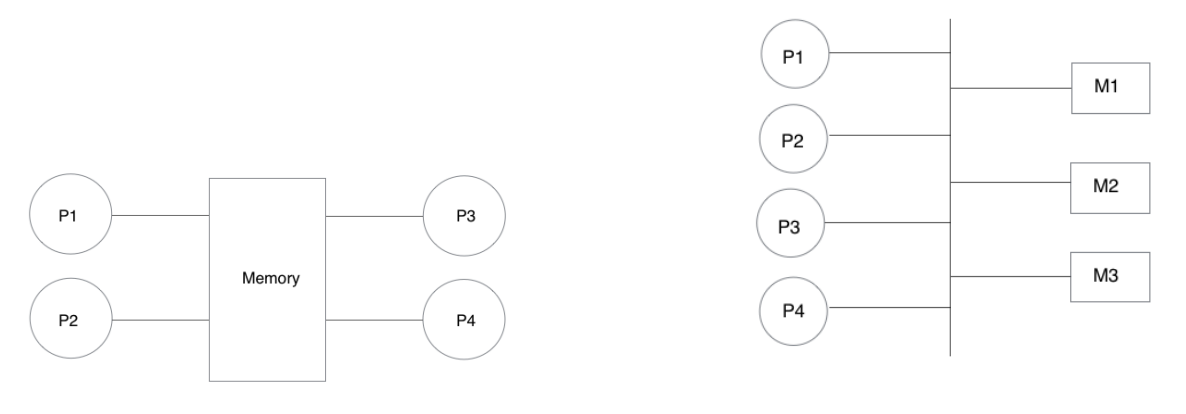
\includegraphics[width=.8\textwidth]{../images/cme323/1.png}
\label{Examples of PRAM}
\end{center}

In practice, either \textbf{arbitrary} or \textbf{garbage} is used.
\subsection{Defenestration of bounds on runtime}
\label{sec:org0f02bd7}
In a PRAM, we have to wait for the slowest processor to finish all of its computation before we
can declare the entire computation to be done. This is known as the \textbf{depth} of an algorithm. We
define
 \begin{align*}
T_1&=\text{amount of (wall-clock) time algorithm takes on one processor}\\
T_p&=\text{amount of (wall-clock) time algorithm takes on \(p\) processors}
 \end{align*}
\subsection{Practical implications of work and depth}
\label{sec:orgff0e276}
\begin{definition}[Work]
The \textbf{work} of an algorithm is defined to be the amount of time required complete all computations
times the number of processors used.
\end{definition}

\textbf{Fundamental lower bound \(T_p\)}:
\begin{equation*}
\frac{T_1}{p}\le T_p
\end{equation*}
\subsection{Representing algorithms as DAG's}
\label{sec:org095ce42}
\textbf{Constructing a DAG from an algorithm}: Specifically, each fundamental unit of computation is
represented by a node. We draw a directed arc from node \(u\) to node \(v\) if
computation \(u\) is required as an \textbf{input} to computation \(v\).

\textbf{Operations in different layers of a DAG can \emph{not} be computed in parallel}. W.L.O.G., we will
assume our DAG is a tree, so the levels of the tree are well-defined. Let the root of the tree
have depth 0. Suppose \(m_i\) denotes the number of operations performed in level \(i\) of the
DAG. Each of the \(m_i\) operations

\textbf{How an algorithm is executed with an unlimited number of processors} At each level \(i\), if
there are \(m_i\) operations we may use \(m_i\) processors to compute all results in constant
time. So with an infinitude of processors, the compute time is given by the depth of the tree.
We then define \textbf{depth} to be
 \begin{equation*}
T_\infty=\text{depth of computation DAG}
 \end{equation*}
\subsection{Brent's theorem}
\label{sec:org0a0731e}
\begin{theorem}[]
With \(T_1,T_p,T_\infty\) defined as above, if we assume optimal scheduling, then
\begin{equation*}
\frac{T_1}{p}\le T_p\le \frac{T_1}{p}+T_\infty
\end{equation*}
\end{theorem}

\begin{proof}
On level \(i\) of our DAG, there are \(m_i\) operations. Hence \(T_1=\sum_{i=1}^nm_i\) where \(T_\infty=n\).
For each level \(i\) of the DAG, the time taken by \(p\) processors is given by
\begin{equation*}
T_p^i=\ceil{\frac{m_i}{p}}\le\frac{m_i}{p}+1
\end{equation*}
\end{proof}
\subsection{Parallel summation}
\label{sec:org8c7ceb8}
\(T_1=n\). We may partition the integers in each level, therefore
\begin{equation*}
T_p\le\frac{n}{p}+\log_2n
\end{equation*}
\(\log_2n\) is just like \(\log_mn\) with some constant \(m\).
\section{Scalable algorithms, Scheduling, and a glance at All Prefix Sum}
\label{sec:org846260a}
\subsection{Types of scaling}
\label{sec:org79334a4}
Another fundamental quantity to understand is the idea of how much speed-up we can hope to
achieve given more processors. There are three different types of scalability:(1) Strong
Scaling, (2) Weak Scaling, and (3) Embarrassingly Parallel

Let \(T_{1,n}\) denote the run-time on one processor given an input of size \(n\). Suppose we
have \(p\) processors. We define the speed up of a parallel algorithm as
\begin{equation*}
\texttt{SpeedUp}(p,n)=\frac{T_{1,n}}{T_{p,n}}
\end{equation*}

\begin{definition}[Strongly Scalable]
If \(\texttt{SpeedUp}(p,n)=\Theta(p)\), we say that the algorithm is \textbf{strongly scalable}
\end{definition}

\begin{proposition}[]
The parallel sum of \(n\) numbers on \(p\) processors is strongly scalable
\end{proposition}

\begin{proof}
\(T_1=n\), \(T_\infty=\log_2n\), so \(\texttt{SpeedUp}(p,n)=\frac{n}{\frac{n}{p}+\log_2n}=\Theta(p)\).
Specifically, both \(n\) and \(p\) are assumed to be going to infinity, but \(p\) grows much
slower than \(n\), hence
\begin{equation*}
\frac{n}{\frac{n}{p}+\log_2n}\ge\frac{n}{\frac{n}{p}+\frac{n}{p}}\ge\frac{p}{2}
\quad\text{ and }\quad
\frac{n}{\frac{n}{p}+\log_2n}\le\frac{n}{\frac{n}{p}}=p
\end{equation*}
\end{proof}

Note that we have used Brent's theorem to derive the scaling bounds. But Brent's theorem assumes
optimal scheduling, which is NP-hard. Fortunately, the existence of a polynomial time constant
approximation algorithm for optimal scheduling implies that these bounds still hold.

\begin{definition}[Weakly Scalable]
If \(\SpeedUp(p,np)=\Omega(1)\), then our algorithm is \textbf{weakly scalable}
\end{definition}

This metric characterizes the case where, for each processor we add, we add more data as well.

\begin{definition}[Embarrassingly Parallel]
When the DAG representing an algorithm has 0-depth, the algorithms is said to be \textbf{embarrasingly parallel}.
\end{definition}
\subsection{Scheduling}
\label{sec:org0a58389}
Given a DAG of computations, at any level in the DAG there are a certain number of computations
which can be required to execute (at the same time). The number of computations is not necessarily
equal to the number of processors you have available to you, so you need to decide how to assign
computations to processor—this is what is referred to as scheduling.
\subsubsection{Problem definition}
\label{sec:org74a455f}
\begin{notation}[]
We assume that the processors are identical. More formally, we are given \(p\) processors and an
unordered set of \(n\) jobs with processing times \(J_1,\dots,J_n\in\R\). Say that the final schedule
for processor \(i\) is defined by a set of indices of jobs assigned to processor \(i\). We call
this set \(S_i\). The load for processor \(i\) is therefore \(L_i=\sum_{k\in S_i}J_k\). The goal is to
minimize the \textbf{makespan} defined as \(L_{\max}=\max_{i\in\{1,\dots,p\}}L_i\)
\end{notation}
\subsubsection{The simple (greedy) algorithm}
\label{sec:orgac7c7d1}
Take the jobs one by one and assign each job to the processor that has the least load at that time.
\subsubsection{Optimality of the greedy approach}
\label{sec:org3fee125}
In either of the cases, where jobs have dependencies or must be scheduled online, the problem is
NP hard. So we use approximation algorithms. We claim that the simple algorithm has an
\textbf{approximation ratio} of 2. For this analysis, we define the optimal makespan to be OPT and try to
compare the output of the greedy algorithm to this. We also define \(L_{\max}\) as above to be
the makespan

\begin{claim}
Greedy algorithm has an approximation ratio of 2
\end{claim}

\begin{proof}
Obviously, \(OPT\ge\frac{1}{p}\sum_{i=1}^nJ_i\), and \(OPT\ge\max_iJ_i\)

Now consider running the greedy algorithm and identifying the processor responsible for the
makespan of the greedy algorithm. Let \(J_t\) be the load of the last job placed on this
processor. Before the last job was placed on this processor, the load of this processor was
thus \(L_{\max}-J_t\). Therefore, all other processors \emph{at this time} must have load at
least \(L_{\max}-J_t\), i.e., \(L_{\max}-J_t\le L_i'\) for all \(i\). Hence summing the inequality
over all \(i\)
\begin{equation*}
p(L_{\max}-J_t)\le\sum_{i=1}^pL_i'\le\sum_{i=1}^pL_i=\sum_{i=1}^nJ_i
\end{equation*}

Therefore
\begin{equation*}
L_{\max}\le\frac{1}{p}\sum_{i=1}^nJ_i+J_t\le OPT+OPT=2OPT
\end{equation*}
\end{proof}

\textbf{What if we could see in the future?} We note that if we first sort the jobs in descending order
and assign larger jobs first, we can naively get a 3/2 approximation. If we use the same
algorithm with a tighter analysis, we get a 4/3 approximation.

\textbf{What's realistic?}
\section{All Prefix Sum}
\label{sec:org1df53dc}
Given a list of integers, we want to find the sum of all prefixes of the list, i.e., the
running sum. We are given an input array \(A\) of size \(n\) elements long. Out output is of
size \(n+1\) elements long, and its first entry is \textbf{always} zero. As an example,
suppose \(A=[3,5,3,1,6]\), then \(R=\AllPrefixSum(A)=[0,3,8,11,12,18]\)
\subsection{Algorithm Design}
\label{sec:org6345776}
\begin{algorithm}
\caption{Prefix Sum}
\begin{algorithmic}[1]
%\State \textbf{Input}: All prefix sum for an array \(A\)
\If{size of \(A\) is 1}
    \State \textbf{return} only element of \(A\)
\EndIf
\State Let \(A'\) be the sum of adjecent pairs
\State Comput \(R'=\AllPrefixSum(A')\)
\State Fill in missing entries of \(R'\) using another \(\frac{n}{2}\) processors
\end{algorithmic}
\end{algorithm}

The general idea is that we first take the sums of adjacent pairs of \(A\). So the size
of \(A'\) is exactly half the size of \(A\).

To compute the running sum for elements whose index is of odd parity in \(A\), i.e., set
\begin{equation*}
r_i=r_{i-1}=a_i
\end{equation*}
for \(i=1,3,5,\dots\) where we by convention let \(r_0=0\)
\subsection{Algorithm Analysis}
\label{sec:orgfb9f726}
\textbf{Pairing entries}: in line 5, where we let \(A'\) be the sum of adjecent pairs, we must
perform \(n/2\) summations, hence work is \(O(n)\).

\textbf{Recursive call}: Line 6 is our recursive call, which is fed an input of half the size of \(A\).

\textbf{Filling in missing entries}: In line 7, filling in missing entries, we can assign each of
 the \(n/2\) missing entries of \(R\) to a processor and compute its corresponding value in
 constant time. Hence line 7 has work \(n/2\), and depth \(O(1)\).

\textbf{Total work and depth}: Let \(T_1=W(n)\), and \(T_\infty=D(n)\),
 \begin{align*}
W(n)&=W(n/2)+O(n)\Rightarrow W(n)=O(n)\\
D(n)&=D(n/2)+O(1)\Rightarrow D(n)=O(\log(n))
 \end{align*}
\subsection{Mergesort}
\label{sec:orga1315e8}
Suppose we parallelize the algorithm via the obvious divide-and-conquer approach, the work done
is then
\begin{equation*}
W(n)=2(W/n)+O(n)=O(n\log n)
\end{equation*}
The depth is
\begin{equation*}
D(n)=D(n/2)+O(n)=O(n)
\end{equation*}
By Brent's theorem, we have that
\begin{equation*}
T_p\le O(n\log n)/p+O(n)
\end{equation*}
The bottleneck lies in \texttt{merge}.

How do we merge \(L\) and \(R\) in parallel?

\textbf{Use binary search to find the rank of an element}: Let's call the output of our algorithm \(M\).
 For an element \(x\in R\), define \(\rank_M(x)\) to be the index of element \(x\) in
 output \(M\). For an such element \(x\in R\), we know how many elements (say \(a\)) in \(R\) come
 before \(x\) since we have sorted \(R\). But we don't know immediately.

If we know how many elements (say \(b\)) in \(L\) are less than \(x\), then we know we should
place \(x\) in the \((a+b)^{th}\) position in the merged array \(M\). It remains to find \(b\).
We can find \(b\) by performing a binary search over \(L\). We perform the symmetric procedure
for each \(l\in L\), so for a call to \texttt{merge} on an input of size \(n\), we perform \(n\) binary
searches, each of which takes \(O(\log n)\) time.
\subsection{Parallel merge}
\label{sec:orgbb5e627}
\begin{algorithm}
\caption{Parallel Merge}
\begin{algorithmic}[1]
\State \textbf{Input}: Two sorted arrays \(A,B\) each of length \(n\)
\State \textbf{Output}: Merged array \(C\), consisting of elements of \(A\) and \(B\) in sorted order
\For{each \(a\in A\)}
    \State Do a binary search to find where \(a\) would be added into \(B\)
    \State The final rank of \(a\) given by \(\rank_M(a)=\rank_A(a)+\rank_B(a)\)
\EndFor
\end{algorithmic}
\end{algorithm}

To find the rank of an element \(x\in A\) in another sorted \(B\) requires \(O(\log n)\) work
using a sequential processor. Hence in total, this parallel merge routine
requires \(O(n\log n)\) work and \(O(\log n)\) depth.

Hence when we use \texttt{parallelMerge} in our \texttt{mergeSort} algorithm,
\begin{alignat*}{2}
W(n)&=2W(n/2)+O(n\log n)&&\Rightarrow W(n)=O(n\log^2n)\\
D(n)&=D(n/2)+\log n&&\Rightarrow D(n)=O(\log^2n)
\end{alignat*}
By Brent's Theorem, we get
\begin{equation*}
T_p\le O(n\log^2n)/p+O(\log^2n)
\end{equation*}
so for large \(p\) we significantly outperform the naive implementation.
\subsection{Motivating Cole's mergesort}
\label{sec:org88b764b}
Can we do better than binary sort?

Let \(L_m\) denote the median index of array \(L\). We then find the corresponding index
in \(R\) using binary search with logarithmic work. We then observe that all of the elements
in \(L\) at or below \(L_m\) and all of the elements in \(R\)
at \(\rank_R(\texttt{value}(L_m))\) are at most the value of \(L\)'s median element. Hence if we
were to recursively merge-sort the first \(L_m\) elements in \(L\) along with the
first \(\rank_R(\texttt{value}(L_m))\) elements in \(R\), and correspondingly for the upper
parts of \(L\) and \(R\), we may simply append the results together to maintain sorted order.
This leads us to Richard Cole\cite{doi:10.1137/0217049}. He works out all the intricate details
in this approach nicely to achieve
\begin{align*}
W(n)&=O(n\log n)\\
D(n)&=O(\log n)
\end{align*}
\section{Divide and Conquer Recipe, Parallel Selection}
\label{sec:orgb1ee5c3}
\subsection{General Divide and Conquer Technique}
\label{sec:org3019df4}
\begin{align*}
T_1&=W(n)=aW(\frac{n}{b})+w\\
T_\infty&=D(n)=D(\frac{n}{b})+t
\end{align*}
\subsection{Parallel Quick Selection}
\label{sec:org067af93}
Suppose we have a list of unsorted integers, which we know nothing about. We wish to find
the \(k^{\text{th}}\) largest element of the integers.

Assume that our input array \(A\) has unique elements.

\textbf{Idea}: From the input list \(A\) pick a value at random called a pivot \(p\). For each item
in \(A\), put them into one of two sublists \(L\) and \(R\) s.t.:
\begin{gather*}
x\in L\Leftrightarrow x<p\\
y\in R\Leftrightarrow y>p
\end{gather*}

Note that the rank of \(p\) is \emph{exactly} \(\abs{L}\). To find the \(k^{\text{th}}\) largest
element in \(A\), call it \(z\), note the following:
\begin{center}
If \(\abs{L}<k\), then \(z\notin L\), we discard the values in \(L\).

If \(\abs{L}>k\), then \(z\notin R\). We discard the values in \(R\).
\end{center}

\begin{center}
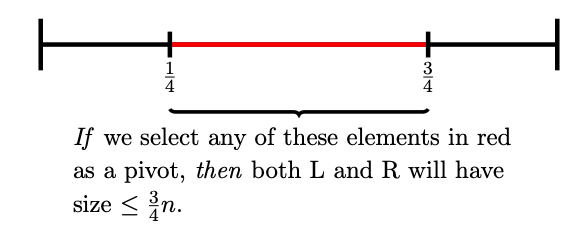
\includegraphics[width=.7\textwidth]{../images/cme323/2.png}
\label{}
\end{center}

So we say that a \textbf{phase} in our algorithm ends as soon as we pick a pivot in the middle half of
our array. Recognize that in phase \(k\), the array size is at
most \(n\left( \frac{3}{4} \right)^k\). The maximum number of \emph{phases} before we can hit a base
case is given by \(\ceil{\log_{4/3}n}\)
\subsection{Analysis - Expected Work}
\label{sec:org66d830e}
Let \(X_k\) denote the number of times \texttt{Select} called with array of input size between
\begin{equation*}
n\left( \frac{3}{4} \right)^{k+1}\le\abs{A}<n\left( \frac{3}{4} \right)^k
\end{equation*}
Total work is given by the sum of the work done for each \(X_k\) multiplied by the number of
calls of that size. Realize that total work done during phase \(k\) given by
\begin{equation*}
X_k\cdot cn\left( \frac{3}{4} \right)^k
\end{equation*}
for some constant \(c\in\R^+\). Total number of phases is \(\ceil{\log_{4/3}n}\). Let \(W\) be a
random variable describing the total work done. Then
\begin{equation*}
W\le\sum_{k=0}^{\ceil{\log_{4/3}n}}\left( X_k\cdot cn\left( \frac{3}{4} \right)^k \right)=
cn\sum_{k=0}^{\ceil{\log_{4/3}n}}\left( X_k\cdot\left( \frac{3}{4} \right)^k \right)
\end{equation*}
We are interested in the expected amount of total work, therefore
\begin{equation*}
\E[W]\le cn\sum_{k=0}^{\ceil{\log_{4/3}n}}\E[X_k]\left( \frac{3}{4} \right)^k
\end{equation*}
We now analyze \(\E[X_k]\). Recall that
\begin{equation*}
\E[X_k]=\sum_{i=0}^\infty i\cdot\Pr(X_k=i)
\end{equation*}

Note that
\begin{equation*}
\Pr(X_k=i)=\left( \frac{1}{2} \right)^{i-1}\cdot\frac{1}{2}=\frac{1}{2^i}
\end{equation*}
Hence
\begin{equation*}
\E[X_k]=\sum_{i=0}^\infty\frac{i}{2^i}=2
\end{equation*}
Ultimately,
\begin{equation*}
\E[W]\le cn\sum_{k=0}^{\ceil{\log_{4/3}n}}\E[X_k]\left( \frac{3}{4} \right)^k\le
2cn\sum_{k=0}^\infty\left( \frac{3}{4} \right)^k=8cn=O(n)
\end{equation*}
So in expectation,
\begin{equation*}
T_1=O(n)
\end{equation*}

\textbf{Applying Markov's Inequality}: We can compute a bound on the probability that our total work
 exceeds a multiple of our expected total work. For example, if we wanted to do analysis that
 our total work will exceed 5 times our expected work:
 \begin{equation*}
P(\text{Total Work}\ge 5\times E[\text{Total Work}])\le\frac{E[\text{Total Work}]}{5\times E[\text{Total Work}]}=\frac{1}{5}
 \end{equation*}
\subsection{Parallelizing our Select Algorithm}
\label{sec:orgc908b1d}
\textbf{Constructing L and R with Small Depth}.

\begin{algorithm}
\caption{Constructing \(L\)(or \(R\))}
\begin{algorithmic}[1]
\State Allocate an empty array of size \(n\), with all value initially 0.
\State Construct indicator list \(B_L[0,\dots,n-1]\) where \(b_i=1\) if \(a_i<p\)
\State Compute \textbf{PrefixSum} on \(B_l\)\Comment{\(O(\log n)\) depth}
\State Create the array \(L\) of size \textbf{PrefixSum}\((B_L[n-1])\)
\For{i=1,2,\dots,n}
    \If{B[i]=1}
        \State \(L[\textbf{PrefixSum}(B_L[i])]\leftarrow a[i]\)\Comment{Can be done in parallel}
    \EndIf
\EndFor
\end{algorithmic}
\end{algorithm}
\begin{equation*}
D(n)=D\left( \frac{n}{4/3} \right)+O(\log n)\Rightarrow D(n)=O(\log^2n)
\end{equation*}
\section{Memory Management and (Seemingly) Trivial Operations}
\label{sec:org427dfe1}
We assume that we can allocate memory in constant time, as long as we don't ask for the meomory
to have special values in it.  That is, we can request a large chunk of memory (filled with
garbage bit sequences) in constant time. However, requesting an array of zeros already
requires \(\Theta(n)\) work since we must ensure the integrity of each entry. In the context of
sequential algorithms, this is not a concern since reading in an input of \(n\) bits, or
outputting \(n\) bits already requires \(\Theta(n)\) work, so zeroing out an array of size n does not
dominate the operation count. However, in some parallel algorithms, no processor reads in the
entire input, so naively zeroing out a large array can easily dominate the operation time of the
algorithm.
\section{QuickSort}
\label{sec:org5376f1d}
\subsection{Analysis on Memory Management}
\label{sec:org4ac3120}
\begin{algorithm}
\caption{QuickSort}
\begin{algorithmic}[1]
\Require An array \(A\)
\Ensure Sorted A
\State \(p\leftarrow\) element of \(A\) chosen uniformly at random
\State \(L\leftarrow[a\mid a\in A,a<p]\)\Comment{Implicitely: \(B_L\leftarrow\bbone\{a_i<p\}^n_{i=1}\), \texttt{prefixSum(\(B_L\))}}
\State \(R\leftarrow[a\mid a\in A,a>p]\)\Comment{which requires \(\Theta(n)\) work and \(O(\log n)\) depth}
\State \textbf{Return} [QuickSort(\(L\)), QuickSort(\(R\))]
\end{algorithmic}
\end{algorithm}

We denote the size of our input array \(A\) by \(n\). To be precise, we can perform step 1
in \(\Theta(\log n)\) work and \(O(1)\) depth. That is, to generate a number uniformly from the
set \(\{1,\dots,n\}\) we can assign \(\log n\) processors to independently flip a bit ``on'' with
probability \(1/2\).

\textbf{Allocating storage for \(L\) and \(R\)}: Start by making a call to the OS to allocate an array
of \(n\) elements; this requires \(O(1)\) work and depth, since we do not require the elements
to be initialized. We compare each element in the array with the pivot, \(p\), and write a 1 to
the corresponding element if the element belongs in \(L\) and a 0 otherwise. This
requires \(\Theta(n)\) work but can be done in parallel, i.e., \(O(1)\) depth. We are left with an
array of 1's and 0's indicating whether an element belongs in \(L\) or not, call
it \(\bbone_L\),
\begin{equation*}
\bbone_L=\bbone\{a\in A:a<p\}
\end{equation*}
We then apply \texttt{PrefixSum} on the indicator array \(\bbone_L\), which requires \(O(n)\) work
and \(O(\log n)\) depth. Then we may examine the value of the last element in the output array
from \texttt{PrefixSum} to learn the size of \(L\). Looking up the last element in array \(\bbone_L\)
requires \(O(1)\) work and depth. We can further allocate a new array for \(L\) in constant time
and depth. Since we know \(\abs{L}\) and we know \(n\), we also know \(\abs{R}=n-\abs{L}\);
computing \(\abs{R}\) and allocating corresponding storage requires \(O(1)\) work and depth.

Thus allocating space for \(L\) and \(R\) requires \(O(n)\) work and \(O(\log n)\) depth.

\textbf{Filling \(L\) and \(R\)}: Now we use \(n\) processors, assigning each to exactly one element in
our input array \(A\), and in parallel we perform the following steps. Each
processor \(1,2,\dots,n\) is assigned to its corresponding entry in \(A\).

Suppose we fix attention to the \(k\)th processor, which is responsible for assigning
the \(k\)th entry in \(A\) to its appropriate location in either \(L\) and \(R\). We first
examine \(\bbone_L[k]\) to determine whether the element belongs in \(L\) or \(R\). In addition,
examine the corresponding entry in \texttt{PrefixSum} output, denote this value
by \(i=\PrefixSum(\bbone_L[k])\). If the \(k\)th entry of \(A\) belongs in \(L\), then it may be
written to the position \(i\) in \(L\) immediately. If the \(k\)th entry instead belongs
in \(R\), then realize that index \(i\) tells us that exactly \(i\) entries ``before''
element \(k\) belong in \(L\). Hence exactly \(k-i\) elements belong in array \(R\) before
element.

The process of filling \(L\) and \(R\) requires \(O(n)\) work and \(O(1)\) depth

Therefore we need \(O(n)\) work and \(O(\log n)\) depth.
\subsection{Total Expected Work}
\label{sec:orgdf669d8}
The level of our computational DAG is \(n\) and there are \(\log_{4/3}n\) levels, therefore
\begin{equation*}
\E[T_1]=O(n\log n)
\end{equation*}

We define the random indicator variable \(X_{ij}\) to be one if the algorithm \emph{does compare}
the \(i\)th \emph{smallest} and the \(j\)th \emph{smallest} elements of input array \(A\) during the course of
its sorting routine, and zero otherwise. Let \(X\) denote the \emph{total} number of comparisons made
by our algorithm. Then we have that
\begin{equation*}
X=\sum_{i=1}^{n-1}\sum_{j=i+1}^nX_{ij}
\end{equation*}
\section{References}
\label{sec:orgb962420}
\label{bibliographystyle link}
\bibliographystyle{alpha}

\label{bibliography link}
\bibliography{../references}
\end{document}
